% !TEX root = ../../report.tex
\section{Evaluation Metrics}
\label{sec:eval-metrics}

%http://www.slideshare.net/gunnar-schroeder

This section will discuss the suitedness of different evaluation metrics in the context
of measuring the recommendation quality for SoBazaar and \emph{G8} of our thesis.

\textbf{G8} automatically disqualifies metrics that consider the ratings themselves as the
ground truth and bases its evaluation score on these numbers. MAE and RMSE can therefore
confidently be crossed off the list of suited metrics.

As for Sobazaar, the main reasons for implementing a recommender system is the desire to improve user
satisfaction and to increase the economic success of a platform. In order to further specify what
defines \emph{good recommendation quality} for SoBazaar, we have to take a closer look at the
recommender's task, the application interface and the data available. The following figures
shows the SoBazaar newsfeed and how the personalized recommendations are to be shown to the user:

\begin{figure}[H]
		\begin{subfigure}[b]{.45\linewidth}
			\centering
	  	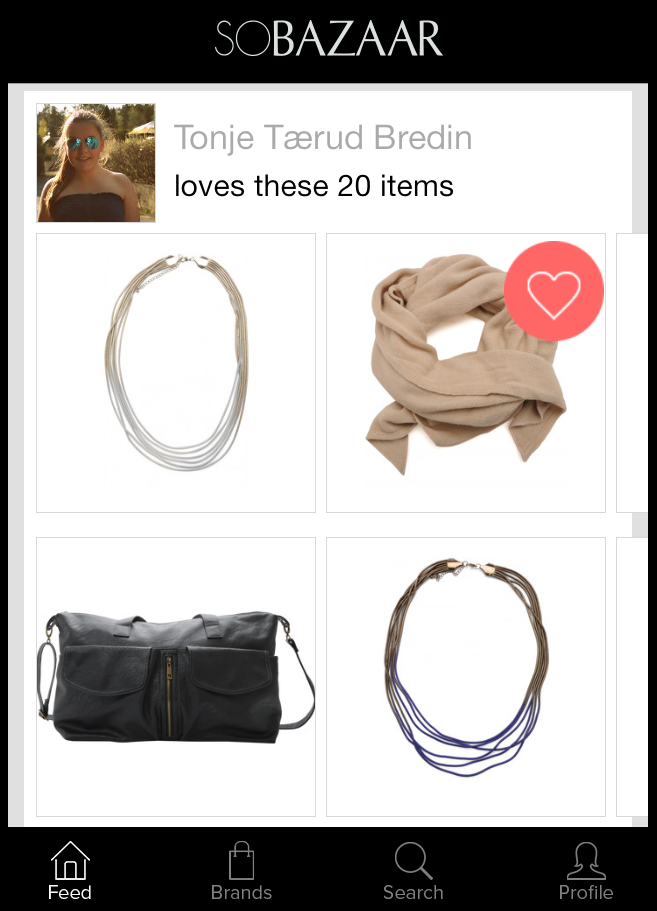
\includegraphics[scale=0.25]{image/SoBazaarfeed2.png}
		\end{subfigure}
		\begin{subfigure}[b]{.45\linewidth}
			\centering
			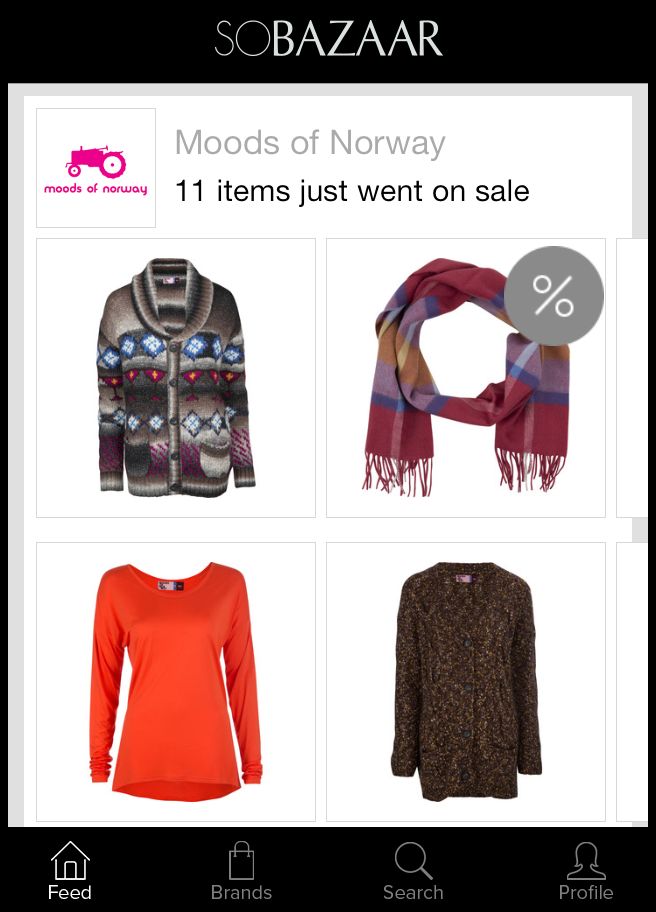
\includegraphics[scale=0.25]{image/SoBazaarsale.png}
		\end{subfigure}
		\caption[Sobazaar News Feed - Version 0.5.1]{SobBazaar news feed items}
		\label{figure:sobazarfeed}
\end{figure}

The most typical task for a e-commerce recommender system is to determine an order of item, often with the
purpose of creating a top-K list of recommendations that is shown in a sidebar or on a dedicated page.
In the case of SoBazaar they are shown in a feed item, showing up to 20 items, making a K value of 20
a natural choice. This makes it safe to assume that the users are more interested in the to ranked items,
than rating predictions for  the entire item collection. Evaluation of top-20 recommendations therefore
suggest a classification or ranking task. An accuracy metric will tell us something the recommenders
ability of retrieving relevant items while a ranking accuracy metric should measure how well the different
methods are at ordering or ranking these predictions. The fact that only 4 recommendations are initially shown,
requiring the user to scroll to view the remaining items highlights the importance of measuring the ranking quality.
We also assume that some items are more relevant than others, e.g. that metric should reward
the recommender for constantly ranking purchases over less relevant events such as clicks.

\subsection{Accuracy Metrics}

Due to the fact that we are working with a highly sparse dataset with a large item collection
it is reasonable to believe the the likeliness of finding a hidden item in the top-20 recommended items
is not very high. We therefore felt that The Area Under Curve (AUC), described in Section \ref{sec:relevance-based}
would be a nice complement to the rank accuracy metrics. AUC allows us to measure the recommenders overall
ability to retrieve relevant items and can therefore be used as a single measure for the overall quality of a recommender
system. Not only considering the top results.

One should be aware of that the AUC scores can be highly inaccurate, especially for cold-start users,
users which the recommender is unable to provide more than a handful of recommendations for. AUC requires
a total ordering of all items not yet rated by the user. This means that the items not recommendable
to the user will be appended in a random order after the known recommendations.
E.g. lets say the recommender is able to generate 10 recommendations for a user out of 4000 items.
The recommender was only able to retrieve one out of two relevant test items. The remaining 3990
items are therefor appended in random order to the users recommendation list. Where the last test item is
appended in the recommendation list can mean the difference between a AUC score of above
0.9 to less than 0.6 if the item is appended at the end of the list, the results can be even more
severe if none of the items is in the initial recommended list, then the results for that user will be
completely random. The most obvious solution to this problem would be to use resampling or to repeat
the experiment multiple times where the order of the items not in the recommendation list are drawn at random and
the results averaged over all the trials.

A frequently uttered point of criticism is that users are often more interested in the items
at the top of a recommendation list but that the AUC measure is equally affected by swaps at the top
or the bottom. Which explains why AUC is not sufficient alone in our case.

\subsection{Rank accuracy}

The introduction gave us two clues that should be considered when selecting a rank accuracy metric.
(1) a ranking accuracy metric that measures the overall ranking is not appropriate, (2) the ranking
metric should be able to account for the different relevance levels.
Again, we assume that we can recommend at most $20$ items for each user at a time. It also pays to submit all $20$
recommendations, because we are not penalized for bad guesses. We also assume that the order matters, so it
is better to submit more certain recommendations first, followed by recommendations we are less sure about.
Which means that we basically select the $20$ best candidates in order. 


Mean average precision $MAP@k$, described in Section~\ref{subp:mean_average_precision_map_} is a popular metric for search
engines and is applied, for example, to report results at the Text Retrieval Conference (TREC). $MAP@20$ will give us a score
of how many items we are able to retrieve and how high up in the recommendation list they are placed. The main weakness in our
case is that it assumes all items to be equally relevant, meaning that it has no way of factoring in the different event types.

Normalized Discounted Cumulative Gain (nDCG) described in Section \ref{subp:normalized_discounted_cumulative_gain_} is a popular metric for
measuring the rank accuracy. It is based on two main assumptions; (1) Highly relevant items are more useful than marginally relevant ones,
(2) The lower the ranked position of a relevant item, the less useful it is for the user, since it is less likely to be \emph{examined}.
The maybe most interesting aspect of nDCG is that it contains an utility function $rel_i$. One can replace the original utility function
and replace it with a function that is more suited to the application. One could e.g. assign the relevance of an item using
the following functions:

\begin{itemize}
\item $rel_i = 1/log(i+k)$: where $i$ is the index of the item in the actual sorted rating list, where $k$ is a constant.
\item $rel_i = u(i)$: simply assign a relevance or utility score such as e.g. the rating of the item or the event type score.
\end{itemize}

The latter would have been perfect, given that we could specify the importance of each event e.g. purchase gets a relevance of 3, want
a relevance of 2 and a click a relevance of 1, as it would give us a single number on the ranking quality of the recommendations.
However, we do not not know these values, meaning that nDCG cannot be used without making assumptions about the importance of the different
event types. To solve this problem we decided to chose a \emph{simpler} approach. We independently measure the recall
and counts of clicks, wants and purchases retrieved by the recommender in the top 20 positions. As you see, it would have been nice to know these
reward attributes to make the evaluation results more \emph{reader friendly}. To check if an user-item touple is a click, want or purchase we create
a file which stores the log events in the following format:


\begin{table}[H]
\centering
\begin{tabular}{*{3}l}
\toprule
UserID	&	ItemID	 &  Event Type  \\ \midrule
11		&	21		 &	1			\\
11		&	101		 &	3			\\
13		&	213		 &	2			\\
13		&	202		 &  3			\\
15		&	202		 &  2			\\
15		&	21		 &  3			\\
\bottomrule
\end{tabular}
\caption{Evaluation - Example event type file}
\label{table:event-type}
\end{table}

For items where a user has multiple events we only use the most \emph{valuable} event. E.g. if a user have both clicked
and purchased an item we store the item as a purchase, giving it a value of 3. When evaluating the recommender we first count the
occurrences of the different events in the test set before looking at the top 20 predictions for each user to see how many of the events in the
different \emph{buckets} was retrieved. In addition we separately measure the $MAP@20$ scores for the different event types to give us some information
about where in the top 20 the items are placed. This gives us the following additional columns for our evaluation metric tables:

\begin{table}[H]
\label{metric-explanation}
	\begin{tabular}{ll}
	\toprule
	$T_{click}$	 	 		& 	Number of click events in the testset \\
	$T_{want}$				&	Number of test events in the testset \\
	$T_{purchase}$	 		&	Number of purchase events in the testset \\
	$P_{click}$		 		&	Number of click events retrieved in the top 20 prediction lists \\
	$P_{want}$		 		&	Number of want events retrieved in the top 20 prediction lists \\
	$P_{purchase}$  		&	Number of purchase events retrieved in the top 20 prediction lists \\
	$R_{click}$				&	$P_{click}$ / $T_{click}$ \\
	$R_{want}$		 		&	$P_{want}$ / $T_{want}$  \\
	$R_{purchase}$	 		&	$P_{purchase}$ / $T_{purchase}$ \\
	$MAP@20_{click}$ 		&	$MAP@20$ considering only click events as relevant items \\
	$MAP@20_{want}$  		&	$MAP@20$ considering only want events as relevant items \\
	$MAP@20_{purchase}$: 	& 	$MAP@20$ considering only purchase events as relevant items \\
	\bottomrule
	\end{tabular}
\end{table}

To illustrate this process more clearly consider the following example where we have
the following test set and prediction lists for three users:

\begin{figure}[H]
		\begin{subfigure}{.5\textwidth}
        \begin{table}[H]
        \centering
        	\begin{tabular}{*{3}l}
        	\toprule
        			UserID	&	ItemID	 &  Rating  	\\ \midrule
        			11		&	21		 &	2			\\
        			11		&	101		 &	5			\\
        			13		&	213		 &	4			\\
        			13		&	202		 &  3			\\
        			5		&	202		 &  5			\\
        			15		&	21		 &  2			\\
        	\bottomrule
        	\end{tabular}
        	\caption{Test set}
        \end{table}
        \end{subfigure}
        \begin{subfigure}{.5\textwidth}
            \begin{table}[H]
            \centering
            	\begin{tabular}{*{3}l}
            	\toprule
            		UserID	&	ItemID	 &  Rating  	\\ \midrule
            		\rowcolor{Gray}
            		11		&	21		 &	5.0			\\
            		11		&	123		 &	3.6			\\
            		\rowcolor{Gray}
            		13		&	213		 &	5.0			\\
            		13		&	1022	 &  4.7			\\
            		15		&	1202	 &  4.4			\\
            		\rowcolor{Gray}
            		15		&	21		 &  4.73		\\
            	\bottomrule
            	\end{tabular}
            	\caption{Prediction set - true positives are highlighted}
            \end{table}
          \end{subfigure}
\end{figure}

We can see that we have an interaction between user 11 and item 21 in our testset and from our event file in
Table~\ref{table:event-type} we can see that the user clicked this item. Similarly we can see that user 15 purchased
item 21 from our event file. Giving us the following event distribution of our test set: $T_{click}$ = 1, $T_{want}$ = 2 and
$T_{purchase}$ = 3.

We then check each user-item touple in our prediction file against our test file, if it is a match we retrieve the
event type for the predictions. Giving us the following $P$ values: $P_{click}$ = 1, $P_{want}$ = 1 and $P_{purchase}$ = 1.
Meaning that we retrieved one of each event type, giving us the following recall score for the different event type:
$R_{click}$ = 1/1, $R_{want}$ = 1/2 and $R_{purchase}$ = 1/3. We can then calculate the different $MAP@20$ scores. E.g. for user 11
the first item in his ranked list is a click meaning that his $AP@20_{click}$ score would be higher than if the item
would have been the third item in his list. The $MAP@20$ numbers can therefore be used as a measure of where in the
top-20 lists the different events can be found. E.g. a high $MAP@20_{purchase}$ score would indicate that the retrieved
purchase events normally are found high up in the top-20 recommendation list and vica versa.

We believe that having the raw counts coupled with the true-postive rate for the different event type and a measure of their
ranking quality will be more informative and give us a clearer overview of the systems performance than using a single rank
metric.


